\chapter{Mon Équipe: Gestion du personnel d'encadrement}\label{chap:team}
\minitoc

\section{Introduction}
L'espace Mon Équipe vous permet d’encoder et de gérer tout votre personnel actif dans les différents secteurs agréés ou reconnus par l’ONE. Cette gestion comprend les relations de travail (contrats, conventions de volontariat) et les qualifications des encadrants.

%\begin{information}
%Cet outil est également utilisé par le Secteur de la Petite Enfance. Dans le cadre de ce guide, nous nous intéresserons uniquement aux fonctionnalités propres à l'Accueil Temps Libre.
%\end{information}

%\begin{remarque}
%Votre administrateur a configuré vos droits d'accès. En fonction de vos droits, vous aurez ou non accès à certains secteurs de l'ATL. Pour en savoir plus, reportez-vous au point \ref{gestion_users} de ce guide. 
%\end{remarque}

\begin{info}
\textbf{Masquer - Activer l'aide contextuel}: 
lors de votre première connexion, une série de messages (‘aide contextuelle’) apparaîtront pour clarifier certains champs ou rappeler des échéances importantes. A tout moment, vous pouvez masquer ces messages, ou les réactiver en passant par le bouton 'Aide' en haut à droite de votre écran. Le bouton Aide contient aussi les données de contact du Service support de l'ONE (cf. remarque \ref{helpdesk}). 
\end{info}


\section{Présentation des écrans}
\subsection{Écran d'accueil}
L'écran d'accueil vous propose deux onglets (voir la figure \ref{fig:main_team}). 
\begin{itemize}
    \item Le premier (\textcolor{bleu}{en bleu}) liste l'ensemble de vos secteurs Accueil Temps Libre pour lesquels vous possédez un agrément.
    \item Le deuxième (\textcolor{vert}{en vert}) liste l'ensemble de votre personnel d'accueil.
\end{itemize}

\begin{info}
\textbf{Affiner des résultats de recherche}: pour chaque cadre, des filtres et des tris vous sont proposés pour vous aider à trouver un secteur ou une personne en particulier. 

\textbf{Pagination des pages}: afin de ne pas alourdir l'écran, les cadres ne vous montrent qu'un nombre limité d'éléments. Vous pouvez en afficher plus au moins avec \textit{'Nombre d'éléments par page'}. Vous pouvez naviguer entre les pages en cliquant sur les < ou >. 
\end{info} 


\begin{figure}
    \centering
    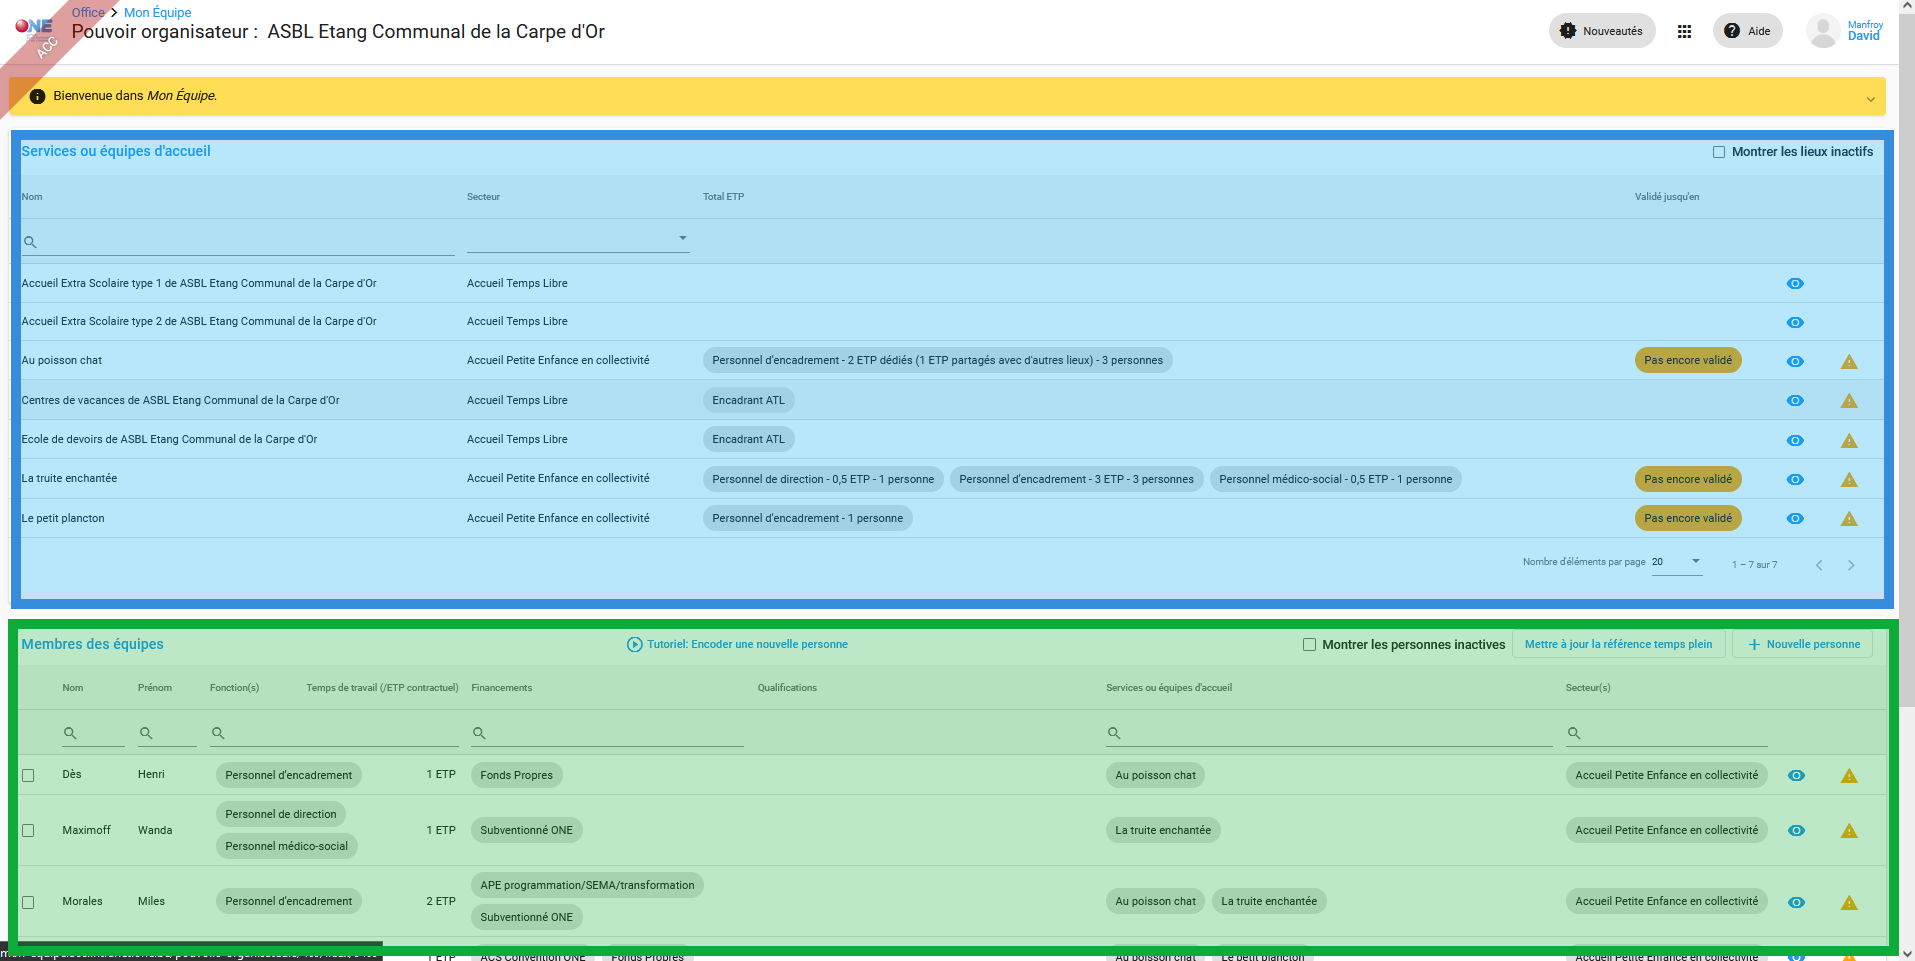
\includegraphics[width=16cm]{Images/team/accueil.png}
    \caption{Écran d'accueil de Mon Équipe}
    \label{fig:main_team}
\end{figure}

\subsection{Écran d'un secteur}\label{team_secteur}
Dans le cadre 1 (en bleu, fig. \ref{fig:main_team}), vous pouvez sélectionner un secteur ATL. Vous aurez alors une vue sur les membres de l'équipe d'encadrement de ce secteur en particulier. Les pages sont paginées et des filtres vous sont proposés. 

Les informations présentées diffèrent d'un secteur à l'autre. 

\begin{itemize}
    \item \textbf{Centres de vacances}: Nom, Prénom, Fonctions, période de vacances, type de centre, Qualification(s) possédées;
    \item \textbf{Écoles de devoirs}: Nom, Prénom, Qualification(s);
    \item \textbf{Accueil extrascolaire}: Nom, Prénom, Qualification(s), Nombre d'heure de formation;
    \item \textbf{Accueil extrascolaire (type2)}: Nom, Prénom, Qualification(s), Fonction(s)Temps de travail (/ETP contractuel),	Financements, Qualifications, Nombre d'heures de formations. 
\end{itemize}

\subsubsection{Personnes inactives}
Par défaut, Mon Equipe ne vous montrera que les personnes qui possèdent un contrat/convention valide en cours. La case \ovalbox{Montrer les personnes inactives} vous permet de voir les personnes dont le contrat/convention ont pris fin. Les personnes qui n'ont pas de date de contrat sont également considérées comme inactives.


\subsection{Écran d'une personne}
La fiche d'une personne est composée de quatre grands onglets (cf. fig. \ref{fig:personne}).

\begin{itemize}
    \item \textbf{Les informations d'identification} (en \textcolor{rouge}{rouge}). En cliquant sur le crayon bleu de modification, vous pouvez corriger des fautes d'orthographe dans les noms et prénoms. 
    
    La mention 'NISS valide (déjà) présent' apparait au lieu du numéro de registre national, afin d'être en conformité avec les règles de sécurité et de RGPD. Si vous avez encodé par erreur le NISS d'une personne avec le nom d'une autre, veuillez contacter notre Service Support via le bouton d'aide.
    
    La date de naissance est automatiquement complétée par déduction du NISS. Veuillez la vérifier et la corriger au besoin, il arrive que le numéro de registre national ne commence pas par la date de naissance.
    
 

    \item \textbf{Les contrats et liens avec le PO} (en \textcolor{orange}{orange})
    \item \textbf{Les qualifications, brevets et autres formations} (en \textcolor{bleu}{bleu})
    \item \textbf{Les prestations, ventilées par secteur} (en \textcolor{vert}{vert})
\end{itemize}


\begin{figure}[H]
    \centering
    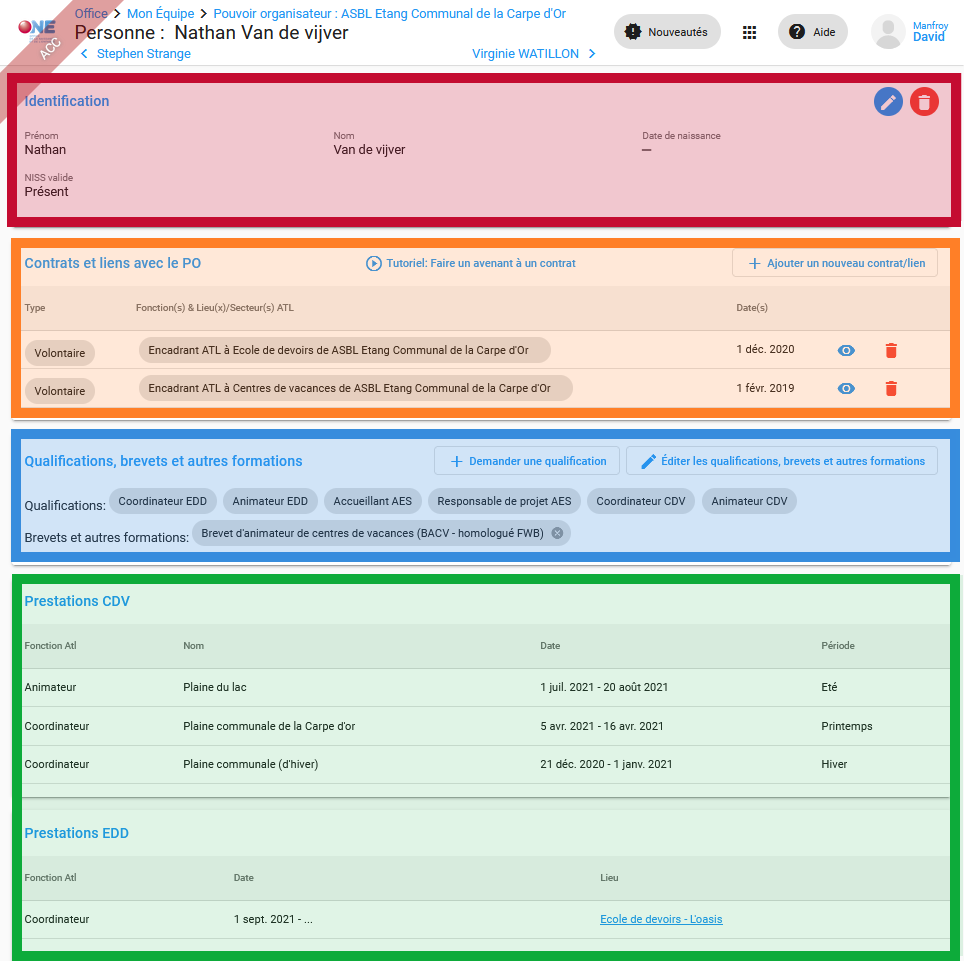
\includegraphics[width=14cm]{Images/team/personne.png}
    \caption{Écran de consultation d'une personne}
    \label{fig:personne}
\end{figure}



\section{Ajouter une personne dans Mon Équipe}\label{team_add_person}
En cliquant sur \ovalbox{ + Nouvelle personne}. Vous serez invité à compléter les données d'identification de la personne. 

\begin{itemize}
    \item Encodez le NISS de la personne. 
    \item Deux cas de figures peuvent se présenter: 
    \begin{itemize}
        \item La personne est inconnue de l'ONE, complétez soigneusement le prénom, nom et date de naissance.
        \item La personne est connue de l'ONE, encodez le nom de famille. 
        
        \begin{information}
         Nous utilisons la combinaison du numéro de registre national (NISS) et le nom de famille pour vérifier si la personne existe déjà dans notre base de données et ne pas vous demander d’information inutile ni ne créer de doublons.
        \end{information}
        
        Veuillez vérifier que vous encodez correctement le numéro NISS et le nom de famille. 
        
        \begin{attention}
        En cas de message d’erreur bloquant, veuillez contacter le Service Support (via le bouton aide en haut à droite), c’est probablement que la personne (son NISS) existe déjà dans notre base de données, mais que le nom de famille avait été encodé avec une erreur.
        \end{attention}
    \end{itemize}
    \item Cliquez ensuite sur le bouton bleu \ovalbox{Créer la personne} ou \ovalbox{Utiliser cette personne}.
\end{itemize}

\begin{figure}[h]
    \centering
    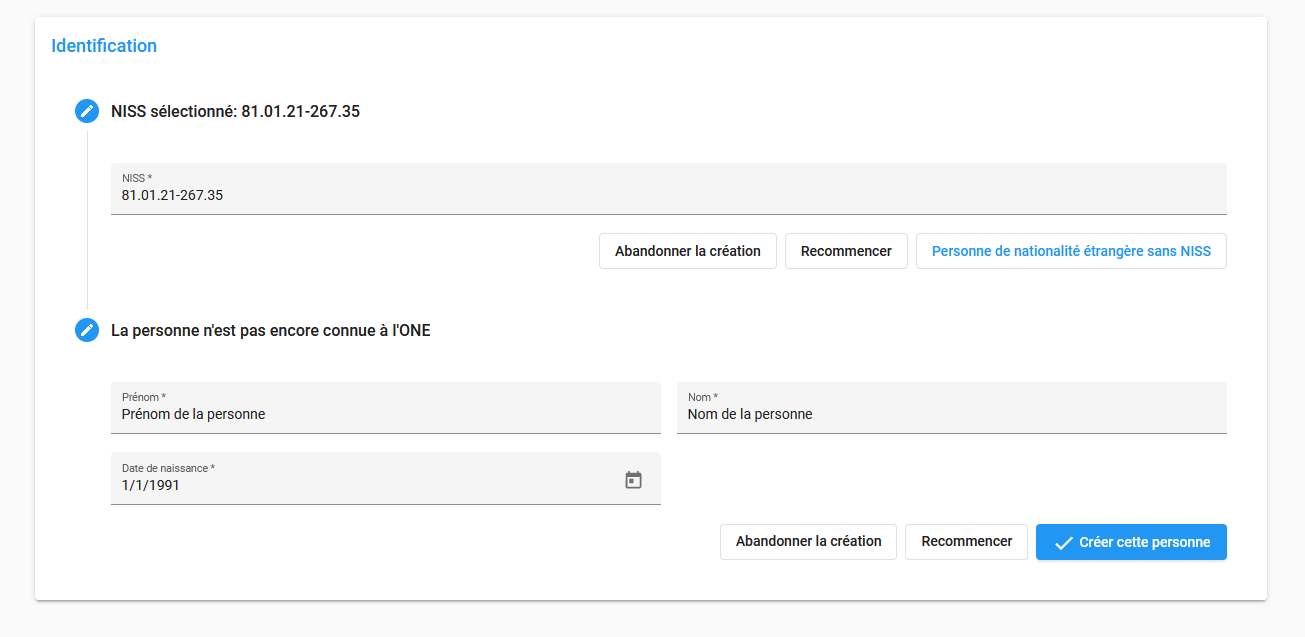
\includegraphics[width=13cm]{Images/team/create_person.png}
    \caption{Fenêtre de création de personne inconnue de l'ONE. Le bouton "créer la personne" est disponible lorsque tous les champs sont complétés.}
    \label{fig:création_personne}
\end{figure}


\section{Ajouter un contrat/un lien}\label{team_add_contract}
Le bouton \ovalbox{+ Ajouter une nouveau contrat/lien} permettra d'assigner la personne à un (ou plusieurs) secteur(s) ATL en renseignant le lien que la personne entretient avec le Pouvoir organisateur.


\subsection{Compléter les données du contrat/lien}
Dans le champ Secteur, sélectionnez "\textbf{Accueil Temps Libre}". 


\subsubsection{Type de relation de travail}
Dans Type de relation de travail, encodez la relation de travail que la personne entretient avec votre Pouvoir organisateur (salarié, volontaire, stagiaire, etc.). Une liste préétablie vous ait proposé en cliquant dans le champ. 

\subsubsection{Temps de travail}
Pour les encadrants des secteurs \textbf{Centres de vacances} et \textbf{Écoles de devoirs}, les données de temps de travail de la convention ne sont pas demandés.


Pour les encadrants du secteur \textbf{Accueil extrascolaire}, vous devez encoder le temps de travail et les dates du contrat (ou convention). 


Pour l'AES2: Mentionnez le temps de travail prévu dans le contrat, même s’il est différent du temps de travail consacré à l’AES2. Complétez également les dates du contrats (ou de la convention)

\subsubsection{Dates du contrat}
Veillez à bien compléter la \textcolor{rouge}{\textbf{date de début}} du contrat ou de la convention de volontariat. Indiquez si nécessaire une date de fin de convention (ou de contrat). Les CDI n'ont pas besoin de date de fin.



\begin{remarque}
 Les encodages de contrat/convention sans date amèneront le système à  considérer les personnes comme étant "inactives". 
\end{remarque}

%\subsection{Pour les contrats AES2}

\subsection{Pour les contrats de travail subventionnés ONE (AES2 et CATL)}\label{ct_travail_aes2}
Lorsque le contrat concerne des secteurs où l'emploi est subventionné, les cadres financement et copie du contrat sont disponibles. 

\subsubsection{Financements}

Si l'emploi de la personne est subventionné par l'ONE, cochez la case "Subventionnable/Subventionné ONE" (AES2) ou "Subventionné ONE" (CATL).

Cette case doit être cochée pour avoir accès à la grille d'encodage des salaires dans les écrans de prestation.

Si la personne reçoit un cofinancement d'un autre organisme ou un financement en fonds propres, cliquez sur \ovalbox{Ajouter un financement}. Vous sélectionnerez alors le type de financement perçu. 

\subsubsection{Copie du contrat}\label{copie_contrat_aes2}
Pour les personnes subventionnées ONE, le dépôt de contrat est obligatoire. Vous chargerez également dans ce cadre tout changement de contrat ou tout avenant au contrat de travail. 




\section{Les Qualifications de la personne}\label{sec:qualif_person}
Pour chaque secteur de l'ATL, il est nécessaire qu'une certaine proportion de vos encadrants soit qualifiée (CDV et EDD) ou entièrement qualifié (AES). C'est à dire, qu'ils répondent aux conditions décrétales requises pour pouvoir exercer un rôle d'animation/d'accueil ou de coordination/responsable de projet.

La figure \ref{fig:personne_qualification} vous montre les qualifications possédées par la personne (en \textcolor{bleu}{bleu}) et la possibilité de demander une qualification (en \textcolor{rouge}{rouge}). Lorsqu'une demande est en cours, elle apparaîtra dans l'encadré \textcolor{bleu}{bleu} avec la mention "\textit{demande en cours"}. 

Pour faire une demande de qualification, cliquez sur \ovalbox{+ Demander une qualification}: 

\begin{itemize}
    \item \textbf{Animateur CDV}: voir le point \ref{ssec:animateur_cdv} (page \pageref{ssec:animateur_cdv});
    \item \textbf{Coordinateur CDV}: voir le point \ref{ssec:coordinateur_cdv} (page \pageref{ssec:coordinateur_cdv});
    \item \textbf{Animateur EDD}: voir le point \ref{ssec:animateur_edd} (page \pageref{ssec:animateur_edd});
    \item \textbf{Coordinateur EDD}: voir le point \ref{ssec:coordinateur_edd} (page \pageref{ssec:coordinateur_cdv});
    \item \textbf{Accueillant AES}:  voir le point \ref{ssec:accueillant_aes} (page \pageref{ssec:accueillant_aes});
    \item \textbf{Responsable de projet AES}:  voir le point \ref{ssec:responsable_aes} (page \pageref{ssec:responsable_aes}).
\end{itemize}

En fonction de la qualification demandée, vous serez invité à encoder une information de \textbf{brevet}, un \textbf{diplôme}, une \textbf{attestation}, une \textbf{équivalence} ou éventuellement une description d'\textbf{expérience utile}. Des \textbf{pièces} (une copie, scan ou une photographie visible) doivent parfois être chargées.

Des espaces de commentaires sont disponibles dans les options afin que vous puissiez transmettre des informations complémentaires à votre agent traitant. Ces commentaires sont facultatifs. 


\begin{remarque}\normalfont
Lorsque la demande est en cours, votre agent traitant va vérifier les pièces justificatives que vous avez soumises. Veillez donc à bien renseigner les informations nécessaires pour le traitement de votre de demande de qualification.

Toute demande \textbf{incomplète} mènera à un refus de la part de votre agent traitant. Vous aurez alors la possibilité de renvoyer la demande avec éventuellement la pièce ou l'information manquante. 
\end{remarque}



\begin{figure}[H]
    \centering
    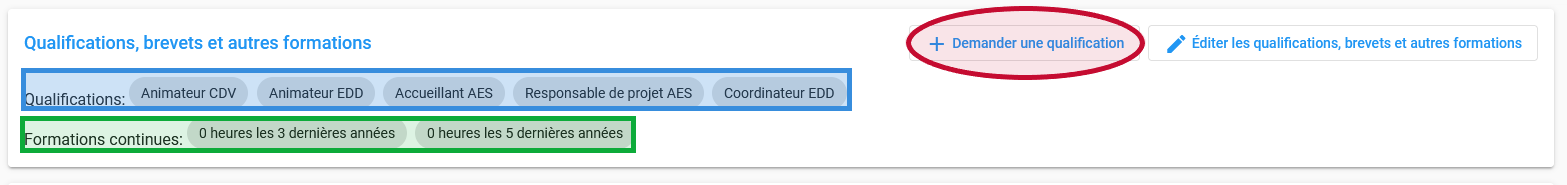
\includegraphics[width=17cm]{Images/team/person-qualif.png}
    \caption{Écran de consultation d'une personne - Cadre qualification}
    \label{fig:personne_qualification}
\end{figure}


\subsection{Animateur CDV}\label{ssec:animateur_cdv}
Il y a quatre possibilités pour acquérir la qualification d'animateur qualifié:
\begin{enumerate}
    \item Détenir le \textbf{brevet d'animateur}\footnote{\label{note:bacv} brevet (BACV) est délivré par un organisme de formation habilité par la FWB au terme d’une formation d’animateur ou de coordinateur de centres de vacances. Attention, les brevets délivrés par le Ministère français de la Jeunesse (BAFA et BAFD) doivent faire l’objet d’une demande d’assimilation ou d'équivalence au préalable.};
    \item Avoir été assimilé et posséder un numéro d'assimilation ;
    \item Demander l'assimilation, c'est-à-dire disposer d'un diplôme du niveau de l'enseignement secondaire à orientation sociale ou pédagogique et avoir effectué 150h d'expérience utile en animation dans un centre de vacances agréé;
    \item Avoir une équivalence au brevet auprès du Service de la jeunesse\footnote{\label{note:equivalence_cdv}Les équivalences sont attribuées par le Service Jeunesse de la Fédération Wallonie-Bruxelles qui transmet un document officiel (document à charger plus bas si en votre possession).

L'équivalence au brevet peut être décernée pour les deux cas suivants :
\begin{itemize}
    \item les anciens brevets ;
    \item les parcours atypiques en animation ou en coordination centres de vacances.
\end{itemize}

Ce parcours doit toujours comporter un minimum de formation de base et d'expérience utile. L’expérience acquise, seule, ne permet pas une équivnce automatique.

Vous souhaitez introduire une demande d’équivalence auprès du service jeunesse de la FWB ? Plus d’infos ici ou au 02/413.24.75 – francoise.cremer@cfwb.be.}.
\end{enumerate}



\subsubsection{Option 1: Brevet d'animateur (BACV)}
Cliquez sur \ovalbox{Encoder le brevet requis}. Ajoutez la date d'octroi; si vous ne la connaissez pas précisément, encodez le au 01/09/'\textit{année d'obtention}'. Si vous disposez d'une copie, chargez-la dans l'espace prévu. Cliquez sur \ovalbox{Enregistrer}. 
    
Cliquez ensuite sur \ovalbox{Demander la qualification}

\subsubsection{Option 2: Numéro d'assimilation déjà octroyé "A1234ANIM"}
Si vous êtes déjà assimilé, vous avez reçu un identifiant de type "A1234 ANIM". Encodez l'identifiant d'assimilation dans le champ "Numéro d'assimilation CDV (si disponible)". Envoyez ensuite la demande. 
    

\subsubsection{Option 3: Demander une assimilation (animateur)}

\vspace*{2mm}
\begin{tcolorbox}[title=Quelles sont les conditions d'assimilation (Animateur) ? ]
Avoir un diplôme ou un certificat de fin d'études à orientation sociale ou pédagogique au moins du niveau de l’enseignement technique secondaire supérieur de promotion sociale ET pouvoir justifier d’une expérience utile de 150 heures de prestation au sein d’un centre de vacances agréé par l’ONE.

\begin{info}
Le nombre d'heures d'expérience est déterminé comme suit :
\begin{itemize}
    \item Séjours et camps : 10 jours consécutifs dont 8 jours pleins correspondent à 150 heures d'expérience utile, 6 jours consécutifs dont 4 jours pleins correspondent à 75 heures d'expérience utile.
    \item Plaines : Seules les journées comprenant au moins 7 heures d'accueil des enfants sont valorisées, 5 journées consécutives de plaine correspondent à 50 heures d'expérience utile.
\end{itemize}
\end{info}

Exemples de diplômes (liste non exhaustive) : AESI, AESS, assistante sociale, éducateur A1, éducateur A2, agent d’éducation, animateur A2, auxiliaire de l’enfance, techniques sociales, puéricultrice, logopède, psychologue, …

\end{tcolorbox}

\textbf{a) Le diplôme}
\\Si un diplôme a déjà été chargé, sélectionnez le dans le tableau des diplômes ou certificats déjà présent.
Sinon ajoutez le diplôme en cliquant sur \ovalbox{Ajouter un diplôme}. Encodez l'intitulé exact du diplôme et sa date d'obtention. Chargez-y une copie dans l'espace prévu à cet effet. Cliquez sur \ovalbox{Enregistrer}.
\begin{attention}
Nous insistons sur l’importance de transmettre un diplôme final et non une attestation de réussite d’un(e) unité/module de formation ou d’une année d’étude. Seuls les diplômes peuvent donner accès à l’assimilation.
\end{attention}


\textbf{b) L'expérience utile}
\\Ajoutez l'expérience utile en cliquant sur \ovalbox{Ajouter une expérience valorisable}. Encoder une description de cette expérience en précisant les dates et centres de vacances agréé où cette expérience a été réalisée. Cliquez sur \ovalbox{Enregistrer}. 

\vspace{0.4cm}
Une fois le \textbf{diplôme} sélectionné et l'\textbf{expérience utile} décrite, cliquez sur \ovalbox{Demander la qualification}
  
  
\subsubsection{Option 4: Équivalence}\label{équivalence_cdv}
Encodez la preuve d'équivalence du Service de la Jeunesse. Dans la petite fenêtre qui s'ouvre, ajoutez la date d'octroi de l'équivalence et chargez une copie dans l'espace prévu. Cliquez ensuite sur \ovalbox{Enregistrer}. 

Cliquez ensuite sur \ovalbox{Demander la qualification}. 


\subsection{Coordinateur CDV} \label{ssec:coordinateur_cdv}
Pour demander la qualification de coordinateur en centres de vacances, il y a 4 possibilités:
\begin{itemize}
    \item Détenir le \textbf{brevet de coordinateur}\footnote{Le brevet de coordinateur de centres de vacances (BCCV) est délivré par un organisme de formation habilité par la FWB au terme d'une formation. Attention, pour les brevets délivrés par le Ministère français de la Jeunesse (BAFD), ceux-ci doivent faire l’objet d’une demande préalable d’assimilation ou d'équivalence.
}.
    \item Avoir été assimilé par le passé (numéro d'assimilation)
    \item Demander l'assimilation, c'est-à-dire disposer d'un diplôme d'enseignement supérieur à orientation sociale ou pédagogique et avoir effectué 250h d'expérience utile en animation et/ou en coordination dans un centre de vacances agréé. Si la personne a déjà été assimilée par le passé, indiquer le numéro d'assimilation.
    \item Avoir une équivalence au brevet auprès du Service de la jeunesse\up{\ref{note:equivalence_cdv}}
\end{itemize}





\subsubsection{Option 1: Brevet de coordinateur (BCCV)}
Cliquez sur \ovalbox{Encoder le brevet requis}. Ajoutez la date d'octroi; si vous ne la connaissez pas précisément, encodez le au 01/09/'\textit{année d'obtention}'. Si vous disposez d'une copie, chargez-la dans l'espace prévu. Cliquez sur \ovalbox{Enregistrer}. 
\subsubsection{Option 2: Numéro d'assimilation déjà octroyé "A1234COOR"}
Si vous êtes déjà assimilé, vous avez reçu un identifiant de type "A1234 COOR". Encodez l'identifiant d'assimilation dans le champ "Numéro d'assimilation CDV (si disponible)". Envoyez ensuite la demande. 


\subsubsection{Option 3: Demander une assimilation (coordinateur)}

\vspace*{2mm}
\begin{tcolorbox}[title=Quelles sont les conditions d'assimilation (Coordinateur) ? ]
Avoir obtenu un diplôme ou un certificat de fin d'études à orientation sociale ou pédagogique du niveau de l’enseignement supérieur social ou pédagogique au moins de type court, de plein exercice ou de promotion sociale ET pouvoir justifier d’une expérience utile de 250 heures de prestation au sein d’un centre de vacances agréé par l’ONE .

\begin{info}
Le nombre d'heures d'expérience est déterminé comme suit :
\begin{itemize}
    \item Séjours et camps : 10 jours consécutifs dont 8 jours pleins correspondent à 150 heures d'expérience utile, 6 jours consécutifs dont 4 jours pleins correspondent à 75 heures d'expérience utile.
    \item Plaines : Seules les journées comprenant au moins 7 heures d'accueil des enfants sont valorisées, 5 journées consécutives de plaine correspondent à 50 heures d'expérience utile.
\end{itemize}
\end{info}

Exemples de diplômes (liste non exhaustive) : AESI, AESS, assistante sociale, éducateur A1, logopède, psychologue, licencié en communication et animation socio-culturelle, licencié en psychologie et sciences de l’éducation, certificat d’aptitudes pédagogiques

N’hésitez pas à nous contacter en cas sur la possibilité d’assimilation d’un diplôme particulier. 

\end{tcolorbox}

\textbf{a) Le diplôme}
\\Si un diplôme a déjà été chargé, sélectionnez le dans le tableau des diplômes ou certificats déjà présent.
Sinon ajoutez le diplôme en cliquant sur \ovalbox{Ajouter un diplôme}. Encodez l'intitulé exact du diplôme et sa date d'obtention. Chargez-y une copie dans l'espace prévu à cet effet. Cliquez sur \ovalbox{Enregistrer}.
\begin{attention}
Nous insistons sur l’importance de transmettre un diplôme final et non une attestation de réussite d’un(e) unité/module de formation ou d’une année d’étude. Seuls les diplômes peuvent donner accès à l’assimilation.
\end{attention}


\textbf{b) L'expérience utile}
\\Ajoutez l'expérience utile en cliquant sur \ovalbox{Ajouter une expérience valorisable}. Encoder une description de cette expérience en précisant les dates et centres de vacances agréé où cette expérience a été réalisée. Cliquez sur \ovalbox{Enregistrer}. 

\vspace{0.4cm}
Une fois le diplôme sélectionné et l'expérience utile décrite, cliquez sur \ovalbox{Demander la qualification}




\subsubsection{Option 4: Équivalence (coordinateur)}
Encodez la preuve d'équivalence du Service de la Jeunesse. Dans la petite fenêtre qui s'ouvre, ajoutez la date d'octroi de l'équivalence et chargez une copie dans l'espace prévu. Cliquez ensuite sur \ovalbox{Enregistrer}. 

Cliquez ensuite sur \ovalbox{Demander la qualification}. 

%\vspace*{2mm}
%\begin{tcolorbox}[title=Comment obtenir une équivalence ?]
%\end{tcolorbox}



\subsection{Animateur EDD} \label{ssec:animateur_edd}
Pour être assimilé comme animateur qualifié : 
\begin{enumerate}
    \item Disposer du brevet d’animateur en Écoles de Devoirs\footnote{La formation au brevet d'animateur en Écoles de Devoirs est organisée par la Fédération francophone des Écoles de devoirs. Le brevet d'animateur est homologué par la Fédération Wallonie Bruxelles.} ou en Centres de Vacances\up{\ref{note:bacv}}.
    \item Disposer d’un certificat d'enseignement secondaire supérieur (CESS) à orientation sociale ou pédagogique, ou d’un diplôme de l’enseignement supérieur;
    \item Avoir une équivalence à ces brevets\footnote{Les équivalences sont délivrées par le Service de la Jeunesse de la FWB, sur base de l’expérience passée valorisable. Toute personne peut demander à faire valoir son expérience acquise et/ou son cursus de formation en vue de bénéficier d’une équivalence au brevet de coordinateur en EDD.
    Pour introduire une demande d'équivalence, contacter le Service de la Jeunesse de la FWB (https://servicejeunesse.cfwb.be/).}.
\end{enumerate}




\subsubsection{Option 1: Brevet d'animateur EDD}
Cliquez sur \ovalbox{Encoder le brevet requis}. Ajoutez la date d'octroi; si vous ne la connaissez pas précisément, encodez le au 01/09/'\textit{année d'obtention}'. Si vous disposez d'une copie, chargez-la dans l'espace prévu. Cliquez sur \ovalbox{Enregistrer}.

\subsubsection{Option 2: CESS (orientation sociale ou pédagogique) ou diplôme de l'enseignement supérieur (toute orientation)}
Si un diplôme a déjà été chargé, sélectionnez le dans le tableau des diplômes ou certificats déjà présent.
Sinon ajoutez le diplôme en cliquant sur \ovalbox{Ajouter un diplôme}. Encodez l'intitulé exact du diplôme et sa date d'obtention. Chargez-y une copie dans l'espace prévu à cet effet. Cliquez sur \ovalbox{Enregistrer}.


\subsubsection{Option 3: Équivalence (animateur EDD)}
Encodez la preuve d'équivalence du Service de la Jeunesse. Dans la petite fenêtre qui s'ouvre, ajoutez la date d'octroi de l'équivalence et chargez une copie dans l'espace prévu. Cliquez ensuite sur \ovalbox{Enregistrer}. 



\subsection{Coordinateur EDD} \label{ssec:coordinateur_edd}
Pour être assimilé comme coordinateur qualifié:
\begin{enumerate}
    \item Posséder un brevet de coordinateur en EDD\footnote{La formation au brevet de coordinateur en Écoles de Devoirs est organisée par la Fédération francophone des Écoles de devoirs. Le brevet de coordinateur est homologué par la Fédération Wallonie Bruxelles.} ou CDV
    \item Posséder un diplôme de l’enseignement supérieur à orientation sociale ou pédagogique
    \item Posséder une équivalence aux brevets EDD\footnote{Les équivalences sont délivrées par le Service de la Jeunesse de la FWB, sur base de l’expérience passée valorisable. Toute personne peut demander à faire valoir son expérience acquise et/ou son cursus de formation en vue de bénéficier d’une équivalence au brevet de coordinateur en EDD.

    Pour introduire une demande d'équivalence, contacter le Service de la Jeunesse de la FWB (https://servicejeunesse.cfwb.be/).}.
\end{enumerate}



\subsubsection{Option 1: Brevet de coordinateur EDD}
Cliquez sur \ovalbox{Encoder le brevet requis}. Ajoutez la date d'octroi; si vous ne la connaissez pas précisément, encodez le au 01/09/'\textit{année d'obtention}'. Si vous disposez d'une copie, chargez-la dans l'espace prévu. Cliquez sur \ovalbox{Enregistrer}.

\subsubsection{Option 2: Diplôme d'enseignement supérieur (orientation sociale ou pédagogique)}
Si un diplôme a déjà été chargé, sélectionnez le dans le tableau des diplômes ou certificats déjà présent.
Sinon ajoutez le diplôme en cliquant sur \ovalbox{Ajouter un diplôme}. Encodez l'intitulé exact du diplôme et sa date d'obtention. Chargez-y une copie dans l'espace prévu à cet effet. Cliquez sur \ovalbox{Enregistrer}.


\subsubsection{Option 3: Équivalence (coordinateur EDD)}
Encodez la preuve d'équivalence du Service de la Jeunesse. Dans la petite fenêtre qui s'ouvre, ajoutez la date d'octroi de l'équivalence et chargez une copie dans l'espace prévu. Cliquez ensuite sur \ovalbox{Enregistrer}. 

\subsection{Demande de qualification: Accueillant AES} \label{ssec:accueillant_aes}
Il existe plusieurs possibilités pour obtenir la qualification d’accueillant AES :


\subsubsection{Option 1: Détenir un \textbf{brevet} d'animateur de centres de vacances (BACV), d'instructeur en éducation physique, de sport et vie en plein air, de moniteur ou d'entraîneur.}

Choisissez le brevet adéquat parmi la liste. Cliquez sur \ovalbox{Encoder le brevet requis}. Ajoutez la date d'octroi; si vous ne la connaissez pas précisément, encodez le au 01/09/'\textit{année d'obtention}'. Si vous disposez d'une copie, chargez-la dans l'espace prévu. Cliquez sur \ovalbox{Enregistrer}.


\subsubsection{Option 2: Détenir un \textbf{diplôme de l’enseignement secondaire à orientation sociale ou pédagogique} à temps plein, en alternance, ou de promotion sociale}
 Exemple : agent d’éducation, animateur, éducateur, puériculteur, auxiliaire de l’enfance en structures collectives ou moniteur pour collectivités d’enfants, auxiliaire de l’enfance, animateur de groupes d’enfants, animateur d’infrastructures locales ;

Si un diplôme a déjà été chargé, sélectionnez le dans le tableau des diplômes ou certificats déjà présents.
Sinon ajoutez le diplôme en cliquant sur \ovalbox{Ajouter un diplôme}. Encodez l'intitulé exact du diplôme et sa date d'obtention. Chargez-y une copie dans l'espace prévu à cet effet. Cliquez sur \ovalbox{Enregistrer}.

\subsubsection{Option 3: Formation initiale de 100h (attestation)}
Avoir suivi la \textbf{formation initiale} accueillant extrascolaire auprès d'un opérateur de formation reconnu/agréé par l'ONE ou auprès d'organisme agréés;

Chargez l'attestation de formation. Cliquez ensuite sur \ovalbox{Demander la qualification}.

\subsubsection{Option 4: Panachage de 100h modules de formations continues suivies sur les notions de base}
Avoir suivi un panachage au moins \textbf{100 heures de formation continue sur les notions de base} de la fonction d’accueillant auprès d'organismes agréés. Il conviendra  de  développer  une  stratégie de formation  cohérente en fonction du parcours de la personne et qui soit diversifié en termes de compétences (pour que l’ensemble des notions de base décrites dans le Décret soient abordées).

Suivez le point \ref{sec:form_cont} du Guide pour ajouter des modules de formations. Après avoir ajouté au minimum 100h de modules de formation suivie. cliquez sur \ovalbox{Demander la qualification}. Votre gestionnaire ira vérifier les modules que vous avez encodés.

\subsection{Responsable de projet d'accueil extrascolaire} \label{ssec:responsable_aes}
Il existe plusieurs possibilités pour obtenir la qualification de responsable de projet AES :

\subsubsection{Option 1: Détenir un brevet de coordinateur de centres de vacances (BCCV), brevet d’aptitude à la gestion de projets et de programmes culturels (BAGIC), coordinateur d’écoles de devoirs.}


Choisissez le brevet adéquat parmi la liste. Cliquez sur \ovalbox{Encoder le brevet requis}. Ajoutez la date d'octroi; si vous ne la connaissez pas précisément, encodez le au 01/09/'\textit{année d'obtention}'. Si vous disposez d'une copie, chargez-la dans l'espace prévu. Cliquez sur \ovalbox{Enregistrer}.


\subsubsection{Option 2: Détenir un diplôme de l’enseignement supérieur au moins de type court, dans une filière sociale, psycho-pédagogique ou d’éducation physique, de plein exercice ou de promotion sociale}

Si un diplôme a déjà été chargé, sélectionnez le dans le tableau des diplômes ou certificats déjà présents.
Sinon ajoutez le diplôme en cliquant sur \ovalbox{Ajouter un diplôme}. Encodez l'intitulé exact du diplôme et sa date d'obtention. Chargez-y une copie dans l'espace prévu à cet effet. Cliquez sur \ovalbox{Enregistrer}.


\section{Formations continues (\textit{ne concerne que l'AES})}\label{sec:form_cont}
Depuis la consultation d'une personne, l'onglet \ovalbox{formation(s)} vous affichera les qualifications reconnues par l'ONE, les justificatifs de qualification (diplôme, brevet, etc.) et les modules de formations continues suivies. Vous aurez également un calcul des heures reconnues et validées par l'ONE. 

\subsection{Heures de formation suivies}
Toutes les formations ne seront pas comptabilisées. Les organismes de formations et les modules de formations encodés depuis la liste déroulante seront automatiquement acceptés.

Par contre, celles qui seront encodées via le choix "Autre" devront passer par une étape de vérification de la part de l'ONE. 

Si la formation n'a pas de lien avec l'Accueil extrascolaire, le module de formation sera "refusé".


\subsection{Ajouter un module de formation continue suivi par une personne}
Pour ajouter un module de formation continue, cliquez sur \ovalbox{+ Encoder une formation continue}. La fenêtre d'ajout du module de formation continue apparaît et vous invite à d'encoder:
\begin{itemize}
    \item \textbf{L'organisme de formation}: la liste vous proposera l'ensemble des organismes agréés et reconnus. Si la liste ne vous propose pas l'organisme, vous pouvez l'encoder en sélectionnant "Autre". 
    \item \textbf{L'intitulé de la formation}: L'ensemble des modules de formations de l'organisme de formation vous sera listé. Si la liste ne vous propose pas le module, vous pouvez l'encoder en sélectionnant "Autre". 
    \item \textbf{la date de début et de fin de formation}: encoder la première date et la dernière date d'organisation du module. Vous devez encoder uniquement les modules qui ont été réellement suivis par la personne; il vous sera impossible par exemple d'ajouter un module de formation qui n'a pas encore été donné.
    \item \textbf{Le nombre d'heures suivies}: par défaut le nombre d'heures du module est celui renseigné dans le catalogue de formation ONE. Vous pouvez encoder un nombre d'heures différent. 
    \item \textbf{l'attestation de présence}: en cliquant sur le petit nuage de chargement, vous pourrez déposer l'attestation. Cette pièce n'est néanmoins pas obligatoire. 
\end{itemize}

Cliquez ensuite sur \ovalbox{Enregistrer}.
Le module de formation suivi est ajouté. 


\subsection{Ajouter un module de formation continue suivi par plusieurs personnes}
Vous avez la possibilité d'ajouter un module de formation suivi pour plusieurs personnes en une seule fois. L'encodage du module se fait alors pour l'ensemble de ces personnes et une ligne de formation continue s'ajoutera pour chacune d'elles.

L'encodage se fait depuis la liste du personnel du secteur Accueil extrascolaire. Cochez les cases des personnes qui ont suivi le module de formation. 

Cliquez ensuite sur \ovalbox{\textcolor{vert}{Encoder des formations pour la sélection}}.

La fenêtre d'ajout du module de formation continue apparaît et vous invite à d'encoder:
\begin{itemize}
    \item \textbf{L'organisme de formation (OF)}: la liste vous proposera l'ensemble des organismes agréés et reconnus. Si la liste ne vous propose pas l'organisme, vous pouvez l'encoder en sélectionnant "Autre". 
    \item \textbf{L'intitulé de la formation}: l'ensemble des modules de formations de l'organisme de formation vous sera listé. Si la liste ne vous propose pas le module, vous pouvez l'encoder en sélectionnant "Autre". 
    \item \textbf{la date de début et de fin de formation}: encoder la première date et la dernière date d'organisation du module. Vous devez encoder uniquement les modules qui ont été réellement suivis par la personne; il vous sera impossible par exemple d'ajouter un module de formation qui n'a pas encore été donné.
    \item \textbf{Le nombre d'heures suivies}:  par défaut le nombre d'heures du module est celui renseigné dans le catalogue de formation ONE. Vous pouvez encoder un nombre d'heures différent. 
\end{itemize}

Cliquez ensuite sur \ovalbox{Enregistrer}.
Le module de formation suivi est ajouté à chacune des personnes sélectionnées. La formation alors ajoutée contiendra la même information (OF, intitulé, dates, heures) pour chaque personne. 


\subsection{Mettre à jour des modules de formation}
\subsubsection{Modifier un module}
En cliquant sur le logo 
\includegraphics[height=0.3cm]{Images/icon/icon-edit.png}, vous avez la possibilité de mettre à jour le module de formation. Pour enregistrer vos modifications, cliquez sur 
\includegraphics[height=0.5cm]{Images/icon/button-maj.png}.

\subsubsection{Supprimer un module de formation}
En cliquant sur le logo 
\includegraphics[height=0.3cm]{Images/icon/icon-del.png}, vous supprimerez le module de formation suivi. Pour confirmer la suppression cliquez sur 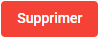
\includegraphics[height=0.5cm]{Images/icon/button-supprimer.png}.



\section{Consulter les prestations dans Mon Équipe}

Dans la consultation d'une personne, seront affichées l'ensemble des prestations de la personne pour l'année en cours (en \textcolor{vert}{vert} dans la figure \ref{fig:personne}). En cliquant sur la prestation, vous serez redirigé vers la gestion de l'activité ou du lieu d'accueil concerné. 